\documentclass[12pt,fleqn]{article}\usepackage{../../common}
\begin{document}
Ders 1-8

Yaylar ve Ağırlıklar (Springs and Masses)

Dersimizin uygulama kısmına geldik. Diyelim ki alttaki gibi bir yay sistemı var,
4 tane yay 3 tane ağırlıktan oluşuyor, ve sonları duvar, tavan gibi bir yerde
sabitlenmiş.

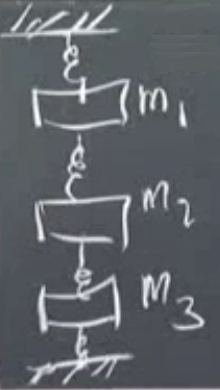
\includegraphics[width=5em]{compscieng_1_08_01.png}

Kütlelerin bir ağırlığı var tabii, ağırlıklar o yaylar aşağı doğru çekiyor, bu
çekim yayları açacak, gerecek, soru yayların ne kadar aşağı ineceği.  Bir yer
değişim (displacement) sorusu bu yani. Unutmayalım yay açılip kapanan bir
mekanizmadır ama açılirken de kapanırken de bir direnç gösterir. Yer değişim en
üstte ve en altta sıfır çünkü oralar sabitlenmiş.

Bir başlangıç hali düşünürsek, diyelim ki yerçekimi o anda etkisiz, ama sonra
yerçekimini bir düğmeye basıp açıyoruz, her yay başlangıç halinden aşağı
doğru bir yer değişimi yaşayacak, 

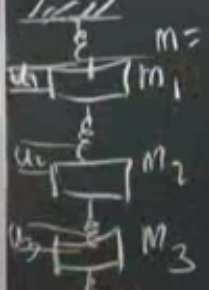
\includegraphics[width=5em]{compscieng_1_08_02.png}

bunlara $u_1,u_2,u_3$ diyebiliriz.

Dikkat salınımı ölçmeye uğraşmıyoruz burada, o daha sonraki derslerde devreye
girecek, zaman faktörünü resme dahil edeceğiz, o sonra. Şimdi sadece kalıcı
durumla ilgileniyorum, yerçekimi açıliyor, yaylar aşağı doğru üzüyor, ve her şey
yerli yerine oturduktan sonra gözlemlenecek yer değişimiyle ilgileniyorum şu
anda.

Her yay parçasının ne kadar uzadığı / esnediği (elongation) ayrı bir ölçüt.
Düşünürsek ikinci kütledeki yer değişimi $u_2$ içinde hem ikinci hem de birinci
yayın esnemesi rol oynar. O yüzden esneme için ayrı bir değişken kullanıyoruz,
$e_1,e_2,e_3$. O zaman kinci yay ne kadar uzar? $u_2-u_1$ kadar. Bir farktan
bahsediyoruz burada. Bazı yaylar sıkışma da yaşayabilir tabii, mesela tahmin
ediyorum ki en alttaki yayda sıkışma olacak.

Tüm bunlar işin geometrik kısmı bir anlamda, yer, uzama, kısalma.. Materyel
faktörlere resme dahil etmek lazım, Hooke Kanunu bunu yapacak. İlk ağırlık
mesela aşağı inerken ilk yayı gerecek. Hooke Kanunu bu noktada der ki yay belli
bir kuvvetle ağırlığı geri çekecek, bu çekiş yayın gerilmesi / uzamasıyla
orantılı olacak. Her yaydaki kuvvete $w_1,w_2,w_3,w_4$ diyelim. Esneme ile ona
karşılık ortaya çıkan kuvvet ilişkisi her materyel için farklı olur, materyele
göre, yay çeşidini göre değisen Hooke yay sabiti bu farklılığı denkleme dahil
edebilir, bu sabitlere $c_1,c_2,c_3,c_4$ diyelim.

Hooke Kanunun lineerdir, ki aşırı fazla olmayan esnemeler için lineerlik
geçerli olacaktır, muhakkak yayı aşırı gerseydik belli bir noktadan sonra
lineer olmayan etkiler görebilirdik, biz bu tür aşırı sonuçlara şu anda
bakmıyoruz.

Devam edelim, Hooke Kanunu der ki her yaydaki kuvvet o yaydaki esnemeyle orantılıdır,

$$
w_i = c_i e_i 
$$

Burada bir köşegen matris görüyorum ben, tüm yaylar, esnemeler, sabitler için

$$
\left[\begin{array}{c}
w_1 \\ w_2 \\ w_3 \\ w_4
\end{array}\right] =
\left[\begin{array}{cccc}
c_1 & & & \\  & c_2 & & \\  & & c_3 & \\ & & & c_4
\end{array}\right]
\left[\begin{array}{c}
e_1 \\ e_2 \\ e_3 \\ e_4
\end{array}\right] 
$$

Ve nihai matris formunda

$$
w = C e
$$

ki $w,C,e$ üstte görülen vektörler ve matris. Materyel kısmı bu şekilde dahil
etmiş olduk, ortadaki sabit matrisi üzerinden. Benzer kanunlar fiziğin diğer
kısımlarında da görülebilir, mesela üstteki $C$ matrisi iletkenliği de temsil
ediyor olabilirdi. Demek istediğim materyel özellikleri denkleme oradan dahil
oluyor. Bu resmi nasıl tamamlarız? Yerçekim bir dış kuvvet, kütleler var, yer
değişimlerine sebep oluyor..

Resmi tamamlamak icin ``kuvvet denge'' denklemi ekleyecegim, her kutle
icin bir denge denklemi olacak.

Not ekleyelim, üstteki türden problem modellemesi pek çok diğer uygulamada ise
yarıyor. Bir geometri var, buradan bir $A$ matrisi çıkartıyoruz, sonra bir
fiziksel adım var, oradan $C$ matrisi geliyor, ve kuvvet dengesi ekleniyor,
resim tamamlanıyor. Kuvvet denge denklemi diğer bir alanda, mesela elektrikte,
Kırchoff Akım Kanunu olabilirdi, ileride ağ yapılarına bakarken göreceğiz, giren
akım çıkan akıma eşit.. Buradaki denge bir yandaki kuvvetin diğer yandakine eşit
olması. Eğer sistemde bir dengeden (equilibrium) bahsedebiliyorsak bir denge
denklemi yazabiliriz demektir.

Şimdi esneme kısmını matris formuna çevirelim. Ne demiştik? Mesela ikinci yay
esnemesi ikinci yer değişimi eksi birinci yer değişimi. Matrissel formda
konuşmak için $e_i$ ve $u_j$  vektörlere lazım, ilişkileri bir matris çarpımı.
Alttaki matriste ikinci satıra ne yazarız?

$$
\left[\begin{array}{c}
e_1 \\ e_2 \\ e_3 \\ e_4
\end{array}\right] =
\left[\begin{array}{cccc}
 & & \\ ? & ? & ? \\  & & \\  & & 
\end{array}\right]
\left[\begin{array}{c}
u_1 \\ u_2 \\ u_3 
\end{array}\right]
$$

O satır sağdaki $u$ vektörü ile çarpılıp sonuçları toplanacak, o zaman
$u_1$ ekşi bir ile, $u_2$ artı bir ile çarpılır, $u_3$ ile ilgilenmiyoruz,
orası sıfır, yani

$$
\left[\begin{array}{c}
e_1 \\ e_2 \\ e_3 \\ e_4
\end{array}\right] =
\left[\begin{array}{cccc}
 & & \\ -1 & 1 & 0 \\  & & \\  & & 
\end{array}\right]
\left[\begin{array}{c}
u_1 \\ u_2 \\ u_3 
\end{array}\right]
$$

Üstte görülen satır bu tür matrislerde tipik bir satırdır. Peki birinci
satır neye benzer? Orada sadece $u_1$ olur, tabii $u_1 - u_0$ farkı
ama ilk yay en üstte sabitlendiği için orada yer değişim olması mümkün
değil $u_0 = 0$, geriye sadece $u_1$ kalıyor.

Üçüncü satır kolay. Dördüncü satırda $u_4$ sabitlenmiş yani sıfır,
tek kalan $-u_3$. Hepsi bir arada,

$$
\left[\begin{array}{c}
e_1 \\ e_2 \\ e_3 \\ e_4
\end{array}\right] =
\left[\begin{array}{rrrr}
1 & 0 & 0 \\ -1 & 1 & 0 \\ 0 & -1 & 1 \\ 0 & 0 & -1
\end{array}\right]
\left[\begin{array}{c}
u_1 \\ u_2 \\ u_3 
\end{array}\right]
\mlabel{1}
$$

Matrise $A$ ismi verirsek, üstteki denklem $e = A u $ olarak belirtilebilir.

Bir adım daha var, kuvvet denge denklemi. Dışarıdan etki eden kuvvet yerçekimi,
$m_1 g$, $m_2 g$, $m_3 g$. Denge için mesela ilk kütleye bakarım, ona hangi
kuvvetler etki eder diye sorarım kendime ve onları dengelemeye uğraşırım.
Bu bana nasıl bir denklem verir acaba?

İlk kütle için kuvvetlere bakarsak, yukarı, aşağı.. Yukarı çeken bir kuvvet
var, yay kuvveti $w_1$. Aşağı çeken $w_2$, değil mi? Alttaki yay her iki
yöne de bir kuvvet uygular. Ayrıca bir de yerçekimi var, $m_1 g$. Hepsi bir
arada

$$
w_1 = w_2 + m_1 g
$$

Diğerleri benzer şekilde,

$$
w_2 = w_3 + m_2 g
$$

$$
w_3 = w_4 + m_3 g
$$

Üsttekini vektör, matris olarak yazmak istiyorum tabii ki, $w$'ların
hepsini sol tarafa geçirirsek işler daha kolaylaşabilir,


$$
w_1 - w_2 = m_1 g
$$

$$
w_2 - w_3 = m_2 g
$$

$$
w_3 - w_4 = m_3 g
$$

Bunlar dış kuvvetler.. Yani (1)'deki iç kuvvetlerle üstteki dış kuvvetleri
dengeleyeceğiz, üstteki $w$'lar iç kuvvetler. Bir matris ortaya çıkacak şimdi.
Önceki numarayı tekrarlarsak,

$$
\left[\begin{array}{rrrr}
1 & -1 & 0 & 0 \\ 0 & 1 & -1 & 0 \\ 0 & 0 & 1 & -1 
\end{array}\right]
\left[\begin{array}{c}
w_1 \\ w_2 \\ w_3 \\ w_4
\end{array}\right] =
\left[\begin{array}{c}
f_1 \\ f_2 \\ f_3
\end{array}\right]
\mlabel{2}
$$

ki $f_i = m_i g$. 

Nasıl ufak adımlarla ilerledik görebiliyoruz herhalde.. Üç adım attık, birinci
adım bizi yer değişimlerinden yaylara götürdü, ikincisi yaylar arasındaki
ilişkilere baktı, üçüncü adımda düğüm noktalara, kütlelere baktık.

Şimdi ana soru şu, üstteki üçüncü adımdaki matris nedir? Onun için yeni bir isme
ihtiyacımız var mı?

Aslında yok. Dikkat edersek (2)'deki matris (1)'dekinin devriği değil mi? Evet!
O zaman ona sadece $A^T$ diyeceğiz.

Üç adımdaki formülleri yanyana koyalım şimdi,

$$
e = Au
\mlabel{3}
$$

$$
w = Ce 
\mlabel{4}
$$

$$
f = A^T w
$$

Bu üç formülü birleştirip nasıl tek formül haline getiririm? Üçüncü formüldeki
$w$ içine ikinci formüldeki $w$'yu sokabilirim, sonra elde edilenin içine
birinci formüldeki $e$'yi sokarım,

$$
f = A^T w = A^T C e = A^T C A u
$$

Nihai sonuç

$$
f = A^T C A u
$$

Tüm yapıyı biraraya getiren formül bu işte, çözmemiz gereken nihai denklem.
Literatürde $A^T C A$'ye direngenlik (stiffness) matrisi adı veriliyor, ve ben
çoğunlukla o matris için $K$ sembolünü kullanırım, yani bu örnek için
$K = A^T C A$ ve çözmemiz gereken sistem $K u = f$.

Bu arada $w$ bilinmiyor, aslında burada iki bilinmeyen, bulmaya uğraştığımız iki
tane fiziksel değişken bloku var, kuvvetler $w$ ve yer değişimleri $e$; bir
köprü, başka bir tür yapı tasarlıyor olabilirdik, onun için yer değişimlerini ve
içsel kuvvetler $w$ değerlerini arıyor olurduk. $w$ ve $u$ değişken öbekleri
birbiriyle yakın ilintili (dual), bazen biri, bazen öteki, ya da ikisiyle aynı
anda iş yapıyor olabiliriz, biraz ileri atlamak oluyor ama sonlu öğeler (finite
element) metodu üstteki formül altyapısını çözer (aslında direngenlik matrisi
kavramı oradan çıkmıştır, şimdi her yerde önümüze çıkıyor).

$A^T C A$ matrisine yakından bakmak bilgilendirici olur; mesela boyutları nedir?
$A$ boyutu 4 x 3, $C$ boyutu 4 x 4, $A^T$ tabii ki 3 x 4, çarpımın sonucu 3 x 3.

Çarpım büyük ihtimalle simetrik, öyle mi bakalım, simetrik demek devriğin
kendisi ile aynı olması demektir, 

$$
(A^T C A)^T = A^T C^T (A^T)^T = A^T C A 
$$

Başlangıca döndük demek ki simetri var.

Şimdi $K = A^T C A$ çarpımına gelelim, onun bulmamız gerekiyor, bu bize tüm
diğer çözümleri zincirleme verecek, $K u = f$ çözüyorsak, çözüm $u = K^{-1}f$.
Eger $u$'yu biliyorsam esnemeyi biliyorum demektir, (3) formulu $e = A u$
idi, o zaman $e = A K^{-1} f$ demektir. Onu alıp (4) içine sokarım, $w = C e$
formülüne, o sonuç ta $w = C A K^{-1} f$. Listeden aşağı indim, hepsi teker
teker çıktı, tabii anahtar ilk çözüm $u = K^{-1} f$.

Ondan önce soralım $K$ çarpımını yapmadan $K^{-1}$ içeriğini açsak,
$K^{-1} = A^{-1}C^{-1} (A^T)^{-1}$ olur ve sağ tarafta bazı hızlı hesaplar
yapabilir miydim acaba? Ne yazık ki $A$ matrisi kare matris olmayabilir ve
bu tür matrislerin tersini almak istemiyorum. 

O zaman $K$ için çarpım yapmamız lazım, yani

$$
K = \left[\begin{array}{rrrr}
1 & 0 & 0 \\ -1 & 1 & 0 \\ 0 & -1 & 1 \\ 0 & 0 & -1
\end{array}\right]
\left[\begin{array}{cccc}
c_1 & & & \\  & c_2 & & \\  & & c_3 & \\ & & & c_4
\end{array}\right]
\left[\begin{array}{rrrr}
1 & -1 & 0 & 0 \\ 0 & 1 & -1 & 0 \\ 0 & 0 & 1 & -1 
\end{array}\right]
\mlabel{5}
$$

Biz altta bu çarpımı hemen \verb!sympy! ile yapalım
  
\begin{minted}[fontsize=\footnotesize]{python}
import sympy aş sp
c1,c2,c3,c4 = sp.symbols('c1 c2 c3 c4')
A = sp.Matrix([[1, 0, 0],
               [-1, 1, 0],
               [0, -1, 1],
               [0, 0, -1]])

C = sp.Matrix([ [c1, 0, 0, 0],
                [0, c2, 0, 0],
                [0, 0, c3, 0],
                [0, 0, 0, c4]  ])

K = A.transpose() * C * A
K
\end{minted}

\begin{verbatim}
Out[1]: 
Matrix([
[c1 + c2,     -c2,       0],
[    -c2, c2 + c3,     -c3],
[      0,     -c3, c3 + c4]])
\end{verbatim}

İşte problemimizi kontrol eden $K$ matrisi bu. Matris kare, simetrik.

Bu tür matrisi daha önce görmüştük değil mi? Üstteki $c_i$ değerlerinin 1
olduğunu farz edin, o zaman $C$ matrisi birim matris olurdu, bu durumda
geriye sadece $A^T A$ kalırdı.

$$
\left[\begin{array}{rrr}
2 & -1 & 0 \\ -1 & 2 & -1 \\ 0 & -1 & 2
\end{array}\right]
$$

Bu matris daha önceki derste gördüğümüz özel $K$ matrisi. 

İki üstteki matris, tekrar yazalım,

$$ K = 
\left[\begin{array}{rrr}
c1 + c2   &     -c2 &       0 \\
-c2       & c2 + c3 &     -c3 \\
0         & -c3     &      c3 + c4
\end{array}\right]
$$

Tüm yay sabitleri bu matris içinde. Üstteki matris hakkında önemli bilgileri
iki üstteki matristen anlayabiliriz. 

$K$ hakkındaki önemli ipuçları nedir? Kare, simetrik dedik, ayrıca pozitif kesin
bir matris. Ve pozitif kesinlik bizi diğer bir özelliğe götürür, bu matrisin
tersi alınabilir.

Peki $K$ matrisi niye pozitif kesin? Hatırlarsak pozitif kesinliğin ana kavramı
pozitif enerji idi. Şu ifade $u^T A^T C A u$ pozitif olmalı, parantezleri 
$(u^T A^T) C (A u)$ şeklinde koyunca belli oluyor, ya da $(u A)^T C (A u)$. 
Ayrıca $Au$ için bir eşitliğimiz var, $Au = e$ o zaman $e^T C e$. Eğer $e,C,e^T$
açık yazarsam,

$$
\left[\begin{array}{rrr}
e_1 & e_2 & e_3 
\end{array}\right]
\left[\begin{array}{rrr}
c_1 &        & \\
    & \ddots & \\
    &        & c_n
\end{array}\right]
\left[\begin{array}{r}
e_1 \\ e_2 \\ e_3
\end{array}\right]
$$

Bu bana $c_1 e_1^2 + c_2 e_2^2 + c_3 e_3^2 + c_4 e_4^2$ verir. Hooke Kanuna
dönerse bir esnetilmiş yaydaki enerji bu karesel formülle hesaplanır. Formülün
esası her şeyi 1/2 ile böler aslında, neyse, ana mesajımız şu, hesaplanan tek
sayı pozitif. Pozitif sayılarla çarpılan karelerin toplamı tabii ki pozitif.

Şimdi Profesör Bathe'nin ADINA adlı o ünlü sonlu öğeler çözen yazılım paketini
düşünürsek, ya da herhangi bir diğer paketi, Ansys, Abaqus gibi, bu paketlerin
odaklandığı büyük resim nedir? Bu paketleri geliştirmek için yıllar geçmiştir,
onlara bir sürü kod eklenmiştir, fakat hepsinin arkasındaki temel fikir sudur,
modeli seç, materyel özellikler (bizim $C$ matrisi) ekle, $K$ matrisini bir
araya getir, nihai adımda sonlu öğeler tekniğiyle sistemi çöz. Her şey $K$
matrisi etrafında dönüyor.


















[devam edecek]

\end{document}


